\section{Tighter \La{} selection}
\label{sec:tight}

The \La{} peak sits on a large combinatorial background (S/B $\approx$ 0.3 within $\pm2\sigma$ with the QA selection), which limits
the precision of its position and makes the \La{} template fits sensitive to the background model. This section tests a tighter
\La{} topological selection, applied identically to data and DDSim templates. \Ks{} is not changed.

\subsection{Choice of the cuts}

\paragraph{Scan.} On run 79509 segments 0--30 (full KFParticle ntuple, KFP mass, $0.5<\pt<4$\gevc;
\fpath{macros/scanLambdaCuts.C}) \ScanNCuts{} combinations of DIRA (0.995--0.9999), $L_{xy}$ (0.5--3~cm), pion and proton
$|{\rm DCA}_{xy}|$ (0.02--0.3 and 0.02--0.1~cm) were evaluated on top of the QA selection. Signal $S$ = counts in
$\pm6$\mevcc{} around the PDG mass minus a linear side-band estimate (1.095--1.104 and 1.128--1.137~GeV/$c^2$), $B$ = that estimate;
figure of merit $S^2/(S+B)$, the effective signal count that sets the error of the peak position. Only cuts that DDSim models are
scanned (no covariance, $\chi^2$ or significance cuts, Sec.~\ref{sec:selection}).
\begin{itemize}
\item QA selection: $S=\ScanBaseS$, $B=\ScanBaseB$, S/B \ScanBaseSB, $S^2/(S+B)=\ScanBaseSeff$.
\item DIRA is the strongest handle: DIRA$>$0.9995 alone gives S/B \ScanDiraSB{} and $S^2/(S+B)=\ScanDiraSeff$ (\ScanDiraKeep\% of
  the signal).
\item A tighter decay length removes signal faster than background: $L_{xy}>2$~cm keeps \ScanLxyKeep\% of the signal
  (S/B \ScanLxySB), because the V0 daughters need silicon hits and therefore decays at small radius.
\item Chosen (\textbf{tight}): QA + DIRA$>$0.9995, $|{\rm DCA}_{xy}(\pi)|>0.10$~cm, $|{\rm DCA}_{xy}(p)|>0.03$~cm: $S=\ScanSelS$
  (\ScanSelKeep\%), $B=\ScanSelB$, S/B \ScanSelSB, $S^2/(S+B)=\ScanSelSeff$ ($\times\ScanGain$). The scan maximum
  (\ScanBestCut, $S^2/(S+B)=\ScanBestSeff$) is within the statistical fluctuation of the scan; the less aggressive DIRA cut was
  preferred (user decision) because the pointing angle is the variable DDSim models least well (Sec.~\ref{sec:open}).
\end{itemize}

\paragraph{Can a tight cut bias the resolution fit?} DDSim applies the selection before the momentum smearing of the fit
(Sec.~\ref{sec:method}). If a tight cut preferentially removed badly measured candidates in data, the data peak would narrow
while the templates would not, and $(a,b)$ would come out too small. Test on the same 31 segments (\fpath{macros/cutBiasTest.C}):
Gaussian width with the QA and the tight selection in data (KFP mass) and in DDSim (templates smeared at the DDSim main point
$a=3.75$\%/(GeV/$c$), $b=1.4$\%, $s=0.991$), for \Ks{} with the same DIRA and pion cuts on both pions and for \La{} with the tight
selection (Table~\ref{tab:tightbias}). The width ratio tight/QA agrees between data and DDSim within the statistics (\Ks{}
\pt-integrated: data $\BiasKsRatD\pm\BiasKsRatDe$, DDSim \BiasKsRatS; \La: $\BiasLaRatD\pm\BiasLaRatDe$ vs \BiasLaRatS). The test
is limited to $\approx$5\% by the 31-segment sample. The DDSim \La{} templates keep \TmplLaTight{} of the candidates
(\TmplLaTightFrac{} of the QA templates).

\begin{table}[H]
\centering\footnotesize
\caption{Cut-bias test on run 79509 segments 0--30: Gaussian width (MeV/$c^2$) with the QA and the tight selection in data
(KFP mass; error of the ratio = quadrature of the two errors, conservative since the tight sample is a subset) and in DDSim at
the main point.}
\label{tab:tightbias}
\begin{tabular}{llcccccc}
\toprule
 & \pt{} (GeV/$c$) & data QA & data tight & data ratio & DDSim QA & DDSim tight & DDSim ratio \\
\midrule
% generated by scripts/make_numbers.py
\Ks & 0.2--0.7 & 4.70$\pm$0.22 & 4.23$\pm$0.15 & 0.899$\pm$0.052 & 4.63 & 4.64 & 1.002 \\
\Ks & 0.7--1.2 & 5.45$\pm$0.32 & 5.47$\pm$0.24 & 1.005$\pm$0.073 & 5.87 & 5.86 & 0.998 \\
\Ks & 1.2--2.2 & 5.95$\pm$0.63 & 6.86$\pm$0.66 & 1.152$\pm$0.165 & 8.39 & 8.23 & 0.981 \\
\Ks & 2.2--4.0 & 7.51$\pm$1.83 & 8.18$\pm$0.27 & 1.090$\pm$0.269 & 13.05 & 12.52 & 0.959 \\
\Ks & 0.2--4.0 & 5.15$\pm$0.17 & 4.94$\pm$0.13 & 0.958$\pm$0.042 & 5.68 & 5.59 & 0.985 \\
\La+$\bar\Lambda$ & 0.5--1.2 & 2.06$\pm$0.30 & 1.90$\pm$0.17 & 0.922$\pm$0.158 & 1.77 & 1.74 & 0.982 \\
\La+$\bar\Lambda$ & 1.2--4.0 & 2.09$\pm$0.53 & 2.21$\pm$0.28 & 1.054$\pm$0.300 & 2.22 & 2.15 & 0.971 \\
\La+$\bar\Lambda$ & 0.5--4.0 & 2.02$\pm$0.27 & 1.99$\pm$0.15 & 0.986$\pm$0.149 & 1.90 & 1.86 & 0.979 \\

\bottomrule
\end{tabular}
\end{table}

\subsection{Production}

The data ntuples of 256 of the 287 segments are not kept (Sec.~\ref{sec:dataset}), so all segments were reprocessed (condor
cluster 481293, \fpath{run3pp/macro/kappa/fill_v0_mass_kappa_v2.C}, \fpath{macro/run_v0mass_kappa_v2.sh}). The v2 fill macro writes,
from the same candidates, all histograms of the first production unchanged, the tight histograms \fcmd{hLa_tight},
\fcmd{hLaBar_tight} in all three mass versions, and a slim candidate tree per segment (pre-selection DIRA$>$0.99,
$L_{xy}>0.2$~cm, $|{\rm DCA}_{xy}|>0.01$~cm; 84~MB for all segments, kept locally in \fpath{data/kappa_v2/v0tree}) so that further
cut variations need no reprocessing. Checks: the v2 macro reproduces the 18 histograms of the first production bin by bin on run
79509 segments 0--30 before submission, and after the production all v1 histograms of all \ReproTwoN{} segments are bin-by-bin
identical to production 480714 (\ChkReproTwo). In \fpath{fitMomRes.C} the option \fcmd{laTight=1} reads the tight data
histograms and applies the same three cuts to the DDSim \La{} templates (\fcmd{rcCosTheta}, \fcmd{rcPiDcaXY}, \fcmd{rcPDcaXY});
the \Ks{} part of the fit is unchanged (identical \Ks{} results: \ChkKsSame).

\subsection{Mass peak}

\begin{figure}[H]
\centering
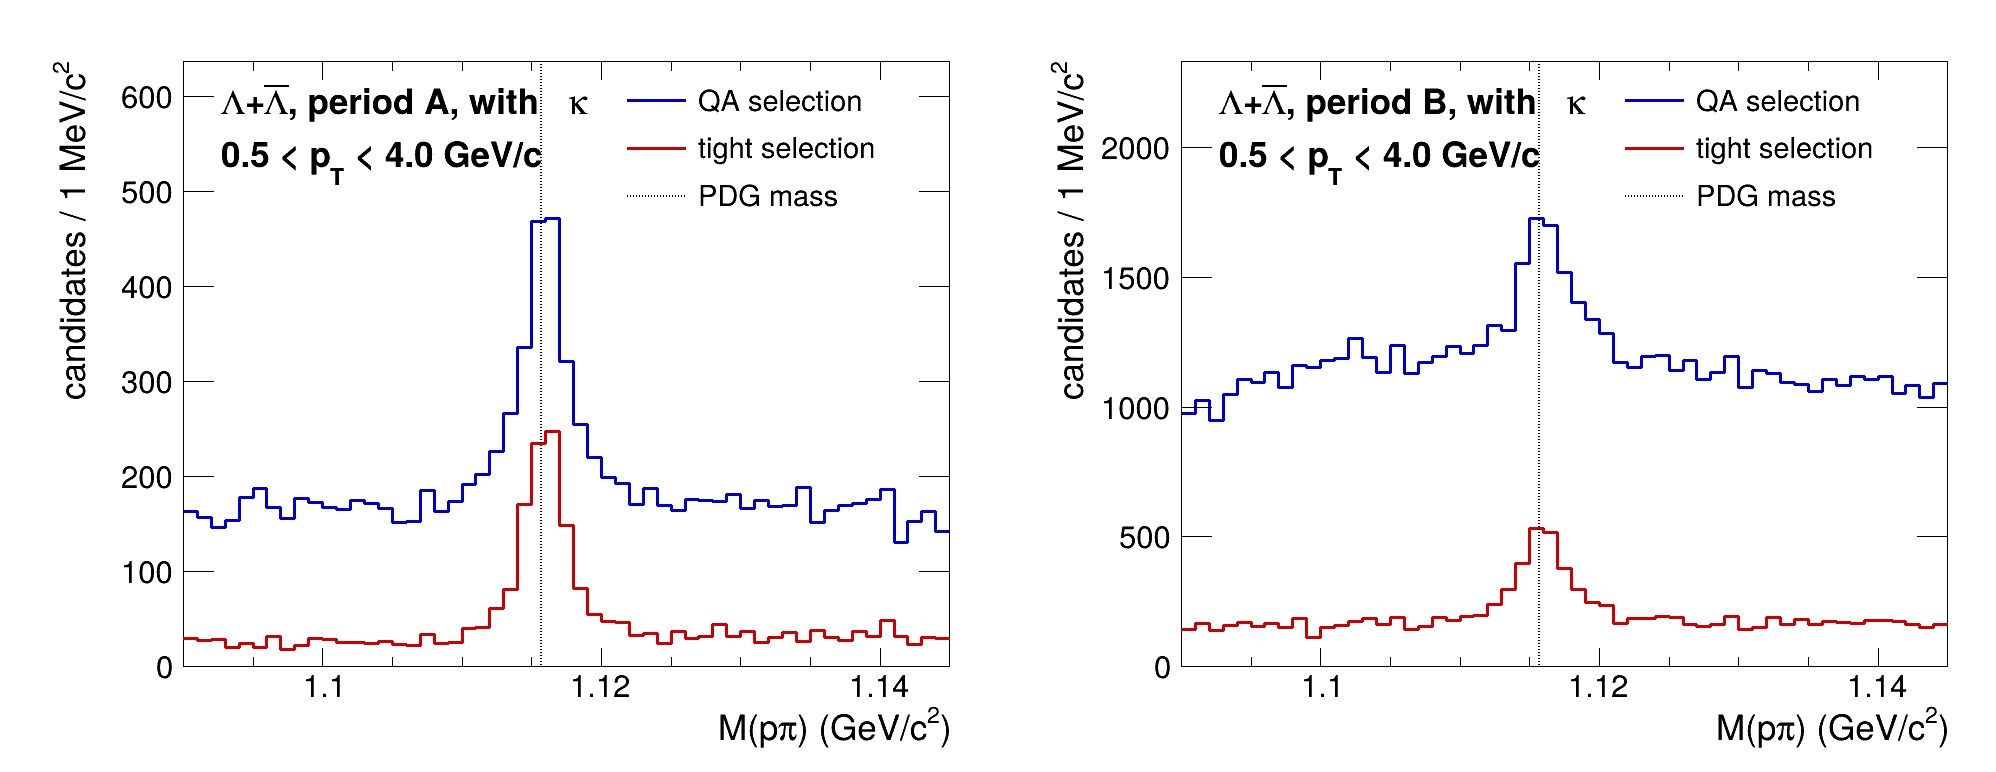
\includegraphics[width=\textwidth]{fig_latight_mass}
\caption{\La+$\bar\Lambda$ mass, recomputed with $\kappa$, $0.5<\pt<4$\gevc, with the QA (blue) and the tight (red) selection;
period A (left) and B (right). Script \fpath{scripts/latight.C}.}
\label{fig:latightmass}
\end{figure}

\begin{table}[H]
\centering\footnotesize
\caption{\La+$\bar\Lambda$ Gaussian peak (gaus + quadratic, 1.103--1.130~GeV/$c^2$, 0.5\mevcc{} bins, likelihood fit),
$0.5<\pt<4$\gevc, QA vs tight selection: mean and width (MeV/$c^2$), S/B within $\pm2\sigma$, and the fraction of the Gaussian
signal kept by the tight cuts. PDG \PdgLa\mevcc. \fpath{macros/laTightPeaks.C}.}
\label{tab:tightpeaks}
\begin{tabular}{llccccccc}
\toprule
 & mass & $M$ QA & $M$ tight & $\sigma$ QA & $\sigma$ tight & S/B QA & S/B tight & kept (\%) \\
\midrule
% generated by scripts/make_numbers.py
A & no $\kappa$ & 1115.55$\pm$0.12 & 1115.65$\pm$0.10 & 2.16 & 2.13 & 0.81 & 3.20 & 71 \\
 & with $\kappa$ & 1115.92$\pm$0.09 & 1115.92$\pm$0.07 & 1.63 & 1.55 & 1.02 & 4.19 & 71 \\
\midrule
B & no $\kappa$ & 1116.24$\pm$0.17 & 1115.93$\pm$0.12 & 2.70 & 2.53 & 0.21 & 0.87 & 57 \\
 & with $\kappa$ & 1116.11$\pm$0.11 & 1115.96$\pm$0.08 & 1.92 & 1.79 & 0.28 & 1.20 & 60 \\
\midrule
all & no $\kappa$ & 1115.99$\pm$0.12 & 1115.81$\pm$0.08 & 2.55 & 2.35 & 0.29 & 1.22 & 61 \\
 & with $\kappa$ & 1116.02$\pm$0.08 & 1115.95$\pm$0.06 & 1.58 & 1.69 & 0.35 & 1.65 & 74 \\

\bottomrule
\end{tabular}
\end{table}

With $\kappa$, the tight selection raises S/B from \PerAllKapLpQaSB{} to \PerAllKapLpTiSB{} (all segments), keeps \PerAllKapLpKeep\%
of the signal (A \PerAKapLpKeep\%, B \PerBKapLpKeep\%) and reduces the error of the peak position from \PerAllKapLpQaMe{} to
\PerAllKapLpTiMe\mevcc{} (A $\PerAKapLpQaMe\to\PerAKapLpTiMe$, B $\PerBKapLpQaMe\to\PerBKapLpTiMe$). The peak stays above the
PDG mass: $\PerAllKapLpTiM\pm\PerAllKapLpTiMe$\mevcc{} (\PerAllKapLpTiAbove\mevcc, $\PerAllKapLpTiPull\sigma$ statistical).

\subsection{Template fits}

\begin{table}[H]
\centering\footnotesize
\caption{\La-only template fit with the QA and the tight \La{} selection, per period and mass version: profile $\Delta\chi^2=1$
intervals, $\chi^2$/ndf, $\Delta\chi^2_\Lambda$ (\La{} $\chi^2$ at the \Ks{} best point minus its minimum), and the joint
\Ks+\La{} best point ($a$ in \%/(GeV/$c$), $b$ in \%, $s$). No best point on the grid edge (\ChkEdgeTight).}
\label{tab:tightfits}
\setlength{\tabcolsep}{3.5pt}
\begin{tabular}{lllccccccc}
\toprule
 & mass & \La{} sel. & $a$ (\%/(GeV/$c$)) & $b$ (\%) & $s$ & $\chi^2$/ndf & $\Delta\chi^2_\Lambda$ & joint $a$, $b$, $s$ \\
\midrule
% generated by scripts/make_numbers.py
A & no $\kappa$ & QA & $4.25^{+0.30}_{-0.18}$ & 1.60 & $0.9910^{+0.0007}_{-0.0009}$ & 293.2/247 & 3.4 & 3.00, 1.60, 0.991 \\
 &  & tight & $4.75^{+0.16}_{-0.18}$ & 1.40 & $0.9930^{+0.0015}_{-0.0012}$ & 244.6/247 & 4.2 & 3.00, 1.60, 0.991 \\
\addlinespace
 & with $\kappa$ & QA & $3.25^{+0.60}_{-0.45}$ & 1.20 & $0.9980^{+0.0022}_{-0.0004}$ & 252.7/247 & 6.1 & 1.50, 1.40, 0.999 \\
 &  & tight & $2.25^{+0.23}_{-0.33}$ & 1.20 & $0.9990^{+0.0014}_{-0.0004}$ & 296.6/247 & 3.4 & 1.50, 1.40, 0.999 \\
\midrule
B & no $\kappa$ & QA & $5.25^{+0.33}_{-0.29}$ & 3.00 & $1.0050^{+0.0009}_{-0.0017}$ & 287.9/247 & 30.5 & 4.00, 1.20, 0.991 \\
 &  & tight & $7.25^{+0.75}_{-0.16}$ & 1.40 & $0.9970^{+0.0021}_{-0.0021}$ & 288.1/247 & 38.3 & 3.75, 1.40, 0.991 \\
\addlinespace
 & with $\kappa$ & QA & $3.50^{+0.16}_{-0.72}$ & 1.40 & $1.0010^{+0.0008}_{-0.0014}$ & 284.0/247 & 4.8 & 2.00, 1.40, 0.998 \\
 &  & tight & $4.25^{+0.52}_{-0.21}$ & 1.20 & $1.0000^{+0.0011}_{-0.0014}$ & 323.9/247 & 11.9 & 2.00, 1.40, 0.998 \\
\midrule
all & no $\kappa$ & QA & $5.25^{+0.52}_{-0.29}$ & 2.00 & $0.9960^{+0.0025}_{-0.0013}$ & 280.5/247 & 25.0 & 3.50, 1.40, 0.991 \\
 &  & tight & $7.75^{+0.14}_{-0.25}$ & 1.00 & $0.9950^{+0.0011}_{-0.0006}$ & 263.5/247 & 45.2 & 3.50, 1.40, 0.991 \\
\addlinespace
 & with $\kappa$ & QA & $2.75^{+0.48}_{-0.63}$ & 1.20 & $1.0000^{+0.0013}_{-0.0011}$ & 255.7/247 & 9.0 & 1.75, 1.40, 0.999 \\
 &  & tight & $4.25^{+0.22}_{-0.31}$ & 1.00 & $0.9990^{+0.0011}_{-0.0003}$ & 309.7/247 & 17.3 & 1.75, 1.40, 0.999 \\

\bottomrule
\end{tabular}
\end{table}

\begin{itemize}
\item \textbf{Scale.} With $\kappa$ and the tight selection the \La-only scale is $s=\PerAKapTiLaS$ (A), \PerBKapTiLaS{} (B)
  and \PerAllKapTiLaS{} (all), consistent with the \Ks{} values (\PerAKapKsS, \PerBKapKsS, \PerAllKapKsS). The half-width of the
  $\Delta\chi^2=1$ interval in $s$ changes from \PerAKapQaLaSW{} to \PerAKapTiLaSW{} (A), \PerBKapQaLaSW{} to \PerBKapTiLaSW{} (B)
  and \PerAllKapQaLaSW{} to \PerAllKapTiLaSW{} (all), in units of $10^{-3}$.
\item \textbf{Resolution, period A.} The tight \La-only curvature term moves towards the \Ks{} value
  ($a=\PerAKapQaLaA\to\PerAKapTiLaA$ vs \Ks{} \PerAKapKsA\%/(GeV/$c$)); $\Delta\chi^2_\Lambda=\PerAKapQaDchi\to\PerAKapTiDchi$.
\item \textbf{Resolution, period B.} The tight \La-only $a$ rises ($\PerBKapQaLaA\to\PerBKapTiLaA$) and the \La/\Ks{} tension grows
  ($\Delta\chi^2_\Lambda=\PerBKapQaDchi\to\PerBKapTiDchi$; all segments $\PerAllKapQaDchi\to\PerAllKapTiDchi$); the \La{} $\chi^2$
  worsens (\PerBKapQaLaChi{} $\to$ \PerBKapTiLaChi/247). Table~\ref{tab:tightwidths}: at 1.2--1.6 and 1.6--2.4\gevc{} the tight data peaks are wider than the tight
  templates at the \Ks{} best point by \WidTiOne{} and \WidTiTwo{} standard deviations of the data width (QA selection:
  \WidQaOne{} and \WidQaTwo).
\item With $\kappa$ the joint \Ks+\La{} best points are unchanged by the tighter \La{} selection (\Ks{} dominates); without
  $\kappa$ the period-B joint point moves by one grid step in $a$ and $b$.
\end{itemize}

\begin{table}[H]
\centering\footnotesize
\caption{\La{} Gaussian width in data / in the template at the \Ks{} best point (MeV/$c^2$), per V0-\pt{} bin, with $\kappa$,
QA vs tight selection (from the template-fit display fits, \fcmd{BIN} rows of the fit logs; ``--'' = data fit unconstrained or at its 0.3\mevcc{} lower limit).}
\label{tab:tightwidths}
\begin{tabular}{llccccc}
\toprule
 & sel. & 0.5--0.9 & 0.9--1.2 & 1.2--1.6 & 1.6--2.4 & 2.4--4.0 \\
\midrule
% generated by scripts/make_numbers.py
A & QA & 2.01$\pm$0.24 / 1.70 & 1.04$\pm$0.10 / 1.48 & 1.73$\pm$0.17 / 1.45 & 1.98$\pm$0.24 / 1.57 & -- / 1.91 \\
 & tight & 1.63$\pm$0.14 / 1.68 & 1.10$\pm$0.07 / 1.44 & 1.47$\pm$0.14 / 1.43 & 1.41$\pm$0.19 / 1.52 & -- / 1.84 \\
\midrule
B & QA & 2.24$\pm$0.32 / 1.74 & 1.39$\pm$0.13 / 1.53 & 1.49$\pm$0.17 / 1.56 & 1.94$\pm$0.19 / 1.77 & 2.08$\pm$0.85 / 2.29 \\
 & tight & -- / 1.70 & 1.32$\pm$0.10 / 1.50 & 1.73$\pm$0.15 / 1.53 & 2.11$\pm$0.20 / 1.72 & -- / 2.19 \\

\bottomrule
\end{tabular}
\end{table}

\begin{figure}[H]
\centering
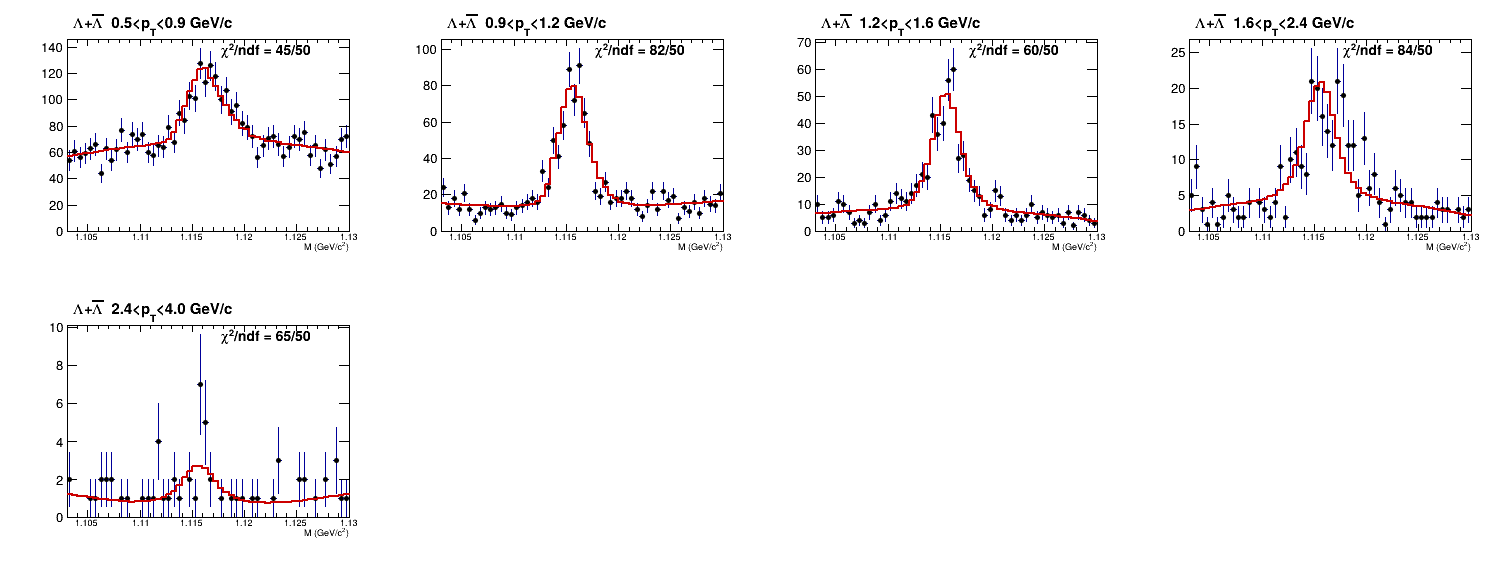
\includegraphics[width=\textwidth]{fig_mass_Lambda_B_tight}
\caption{\La+$\bar\Lambda$ mass, period B, with $\kappa$ and the tight selection; template at the \Ks{} best point (prediction).
Compare Fig.~\ref{fig:masslaB} (QA selection).}
\label{fig:masslaBtight}
\end{figure}

\choice{\textbf{Use of the tight selection} (adopted): the tight \La{} selection is used for the \La{} peak position and the
\La{} momentum scale ($s_\Lambda$ with $\kappa$: \PerAKapTiLaS, \PerBKapTiLaS, \PerAllKapTiLaS{} for A, B, all). The resolution
$(a,b)$ stays determined by \Ks{} (Table~\ref{tab:summary}); the \La{} resolution with the tight selection is not used until the
period-B width mismatch is understood (Sec.~\ref{sec:open}).}

\caveat{Why the tight templates under-predict the period-B width above 1.2\gevc{} is not established. Candidates: the pointing
angle is too good in DDSim (true PV, unsmeared directions; in the full-simulation closure study 5\% of the true \Ks{} have DIRA$<$0.995 against 0.1\% in DDSim), so a
DIRA$>$0.9995 cut selects different decay topologies in data and DDSim; higher pile-up in period B; statistics (the 2.4--4\gevc{}
bin has $\approx$10 tight signal candidates in B). The 31-segment bias test (period A only) shows no effect at the 5\% level.}
